% c4-updatevec.tex

\documentclass{standalone}
% newcommands.tex

\newcommand{\enq}{\texttt{enq}}
\newcommand{\deq}{\texttt{deq}}
\newcommand{\pput}{\texttt{PUT}}
\newcommand{\get}{\texttt{GET}}
\newcommand{\vs}{\texttt{vis}}
\newcommand{\so}{\texttt{so}}
\newcommand{\arb}{\texttt{ar}}
\newcommand{\rf}{\texttt{rf}}

% example
\newcommand{\po}[2]{\draw [->, thick] (#1) to node[above] {\Large{\so}} (#2);}
\newcommand{\pva}[2]{\draw [->, thick] (#1) to node[above] {$\Large{\so},\Large{\vs},\Large{\arb}$} (#2);}
\newcommand{\pbva}[2]{\draw [->, thick] (#1) to node[above] {$\Large{\so}$} node[below] {$\Large{\vs},\Large{\arb}$} (#2);}
\newcommand{\pv}[2]{\draw [->, thick] (#1) to node[above] {\Large{\so}} node[below] {\Large{\vs}} (#2);}
\newcommand{\evis}[2]{\draw [->, thick] (#1) to node[above, sloped, near end] {\Large{\vs}} (#2);}
\newcommand{\mvis}[2]{\draw [->, thick] (#1) to node[above, sloped] {\Large{\vs}} (#2);}
\newcommand{\ar}[2]{\draw [->, thick, allow upside down] (#1) to node[above, sloped] {\Large{\arb}} (#2);}
\newcommand{\va}[2]{\draw [->, thick, allow upside down] (#1) to node[above, sloped] {$\Large{\vs},\Large{\arb}$} (#2);}
\newcommand{\vab}[2]{\draw [->, thick, allow upside down] (#1) to node[below, sloped, near end] {$\Large{\vs},\Large{\arb}$} (#2);}
\newcommand{\vae}[2]{\draw [->, thick, allow upside down] (#1) to node[above, sloped, near end] {$\Large{\vs},\Large{\arb}$} (#2);}
\newcommand{\vas}[2]{\draw [->, thick, allow upside down] (#1) to node[sloped, near start, above] {$\Large{\vs},\Large{\arb}$} (#2);}

% serialization
\newcommand{\scc}[2]{\draw [->, very thick] (#1) to (#2);}
\newcommand{\rva}[2]{\draw [->, thick, allow upside down] (#1) to node[above, sloped] {$\Large{\rf},\Large{\vs},\Large{\arb}$} (#2);}
\newcommand{\rvb}[2]{\draw [->, thick, allow upside down] (#1) to node[below, sloped] {$\Large{\rf},\Large{\vs},\Large{\arb}$} (#2);}


\usepackage{tikz}
\usetikzlibrary{shapes, positioning, arrows.meta, decorations.pathmorphing}

\begin{document}
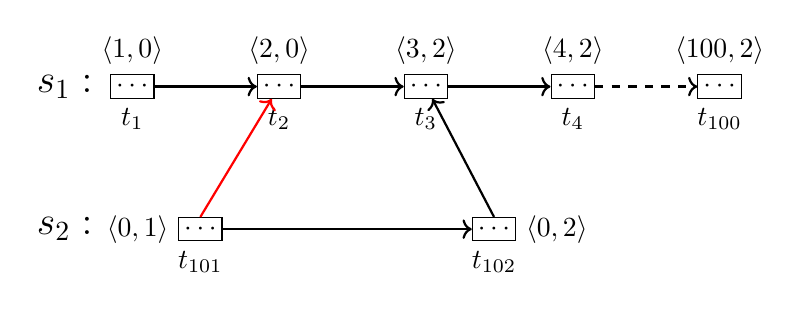
\begin{tikzpicture}[
  node distance = 1.00cm and 1.30cm,
  so/.style = {->, thick},
  wr/.style = {->, thick},
  co/.style = {->, thick},
  vo/.style = {->, thick},
  txn/.style = {draw, inner sep = 2pt}]

  % t1:
  \node[txn,
			label = below : $t_{1}$,
			label = above : {$\langle 1, 0 \rangle$}]
		(t1) {$\cdots$};
  % t2:
  \node[txn, right = of t1,
			label = below : $t_{2}$,
			label = above : {$\langle 2, 0 \rangle$}]
    (t2) {$\cdots$};
  % t3:
  \node[txn, right = of t2,
			label = below : $t_{3}$,
			label = above : {$\langle 3, 2 \rangle$}]
    (t3) {$\cdots$};
	% t4:
  \node[txn, right = of t3,
			label = below : $t_{4}$,
			label = above : {$\langle 4, 2 \rangle$}]
    (t4) {$\cdots$};
	% t100:
  \node[txn, right = of t4,
			label = below : $t_{100}$,
			label = above : {$\langle 100, 2 \rangle$}]
    (t100) {$\cdots$};

	% t101:
  \node[txn, below right = 1.50cm and 0.30cm of t1,
			label = below : $t_{101}$,
			label = left : {$\langle 0, 1 \rangle$}]
    (t101) {$\cdots$};
	% t102:
  \node[txn, below right = 1.50cm and 0.30cm of t3,
			label = below : $t_{102}$,
			label = right : {$\langle 0, 2 \rangle$}]
    (t102) {$\cdots$};

	% session s1
	\node[left = 0.10cm of t1] (s1) {\Large$s_{1}:$};
	\node[] (s2) at (s1 |- t101) {\Large$s_{2}:$};

  % t1-SO-t2
  \draw[so] (t1) to node[above]{$\SO$} (t2);
	% t2-SO-t3
  \draw[so] (t2) to node[above]{$\SO$} (t3);
	% t3-SO-t4
  \draw[so] (t3) to node[above]{$\SO$} (t4);
	% t4-SO-t100
  \draw[so, dashed] (t4) to node[above]{$\SO$} (t100);

	% t101-SO-t102
  \draw[so] (t101) to node[above]{$\SO$} (t102);

	% t101-VO-t2
  \draw[vo, red] (t101.north) to node[sloped, above]{$\CM$} (t2);
  % t102-WR-t3
  \draw[wr] (t102.north) to node[sloped, above]{$\WR$} (t3);
\end{tikzpicture}
\end{document}